\subsubsection{Progress Tracking Tools}
An important point in Scrum is that the Team is a self-managing entity. As evident in the distribution of roles there is no project leader involved (the ScrumMaster should \emph{not} be confused with such), and this requires the Team itself to keep track of progress. The already mentioned Daily Scrum is an important part of this, but there is also other tools available.

\paragraph{Item status}
In a work environment Sprint Backlogs are sometimes maintained as stickers on a big board (called a \textbf{Scrum Board}), which provides an easy overview of the current status. This was not possible (or reliable at least) at our university as we can not reserve the white boards or rooms. Fortunately our online tool has several status states (Unstarted, Started, Finished, Delivered, Approved, and Rejected) for each items, which we made use of.
\begin{figure}[htb]
	\centering
	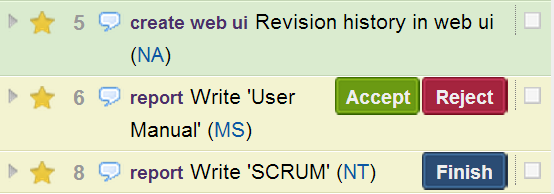
\includegraphics[width=0.50\textwidth]{SCRUM/graphics/status_example.png}
	\caption{An example of statuses on items in the Sprint Backlog. The top story is finished, the second has been delivered (but not yet approved), and the bottom one has been started.}
	\label{fig:itemstatus}
\end{figure}

\paragraph{Daily estimates}
Another common approach to progress tracking in Scrum is to update the Sprint Backlog with daily estimates of the remaining effort (given in points). In Pivotal Tracker this is done by splitting the big items (an \textit{Epic} in Pivotal Tracker terminology) up into lesser related items (\textit{stories} in Pivotal Tracker terminology).
\begin{figure}[htb]
	\centering
	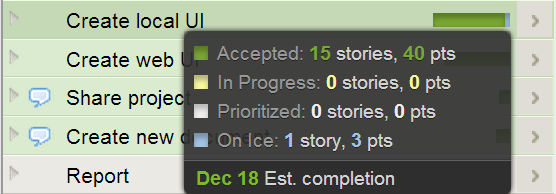
\includegraphics[width=0.50\textwidth]{SCRUM/graphics/epic_example.png}
	\caption{An example of progress tracking on an Epic (Pivotal Tracker terminology)}
	\label{fig:epicexample}
\end{figure}

The last progress tracking tool we've used, which is very common in Scrum-based development, is a  \textbf{Sprint Burndown Chart}. Pivotal Tracker generated this chart (among others) for us, thus making it easy to track how much work was left to be done each Sprint.
\begin{figure}[htb]
	\centering
	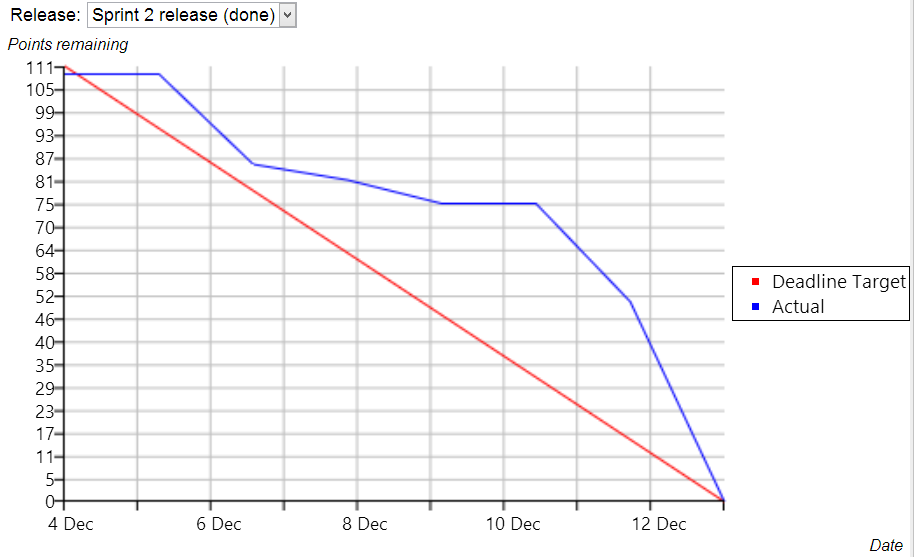
\includegraphics[width=0.75\textwidth]{SCRUM/graphics/burndown_chart.png}
	\caption{Our burndown chart for Sprint 2}
	\label{fig:burndownchart}
\end{figure}